\newpage
\section{Building of TSEngine}
\label{sec:build}
The main purpose of creating sophisticated building system is to assure multiplatform and non-device dependent project, simultaneously easy to set up.\\ This is obligatory in long-living projects and in non-single developer projects.
To fulfill those assumptions the core of every modern C++ project is \hyperref[sec:stack_cmake]{CMake}, this is no different for our project.
Comprehensive series of article about types of libraries in C++ \cite{cpplibs} that knowledge included there may turn out to be useful in this section.
% TODO: dominik the preface of building of tsengine can on the other hand become a fragment of theory, wydt, do you have time?
Unfortunately at this moment \hyperref[sec:problems]{"Problems During the Development"}
\subsection{Build Structure}
\label{sec:build_struct}
\begin{figure}
  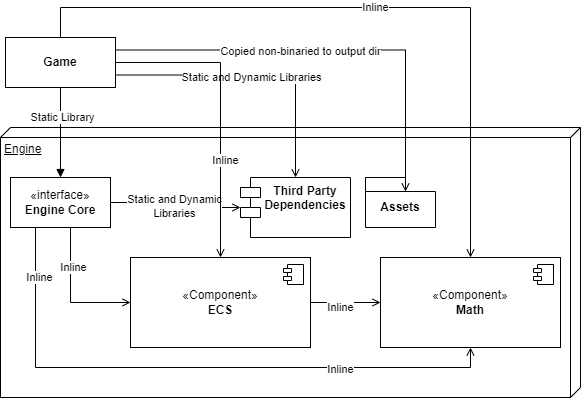
\includegraphics[width=\linewidth]{figures/build.png}
  \caption{Build Structure}
\end{figure}
Currently, TSEngine is delivered to the game in the form of static library, unfortunately at the moment of writing this thesis we haven't yet implemented dynamic version of TSEngine, but we provided abstraction and architecture to do it.
\begin{verbatim}
├───engine
│   ├───CMakeLists.txt
│   └───tests
│       └───CMakeLists.txt
├───external
│   └───CMakeLists.txt
└───game
│   └───CMakeLists.txt
└───CMakeLists.txt
\end{verbatim}
\begin{table}[h]
\caption{CMake files}
\end{table}
\newpage
\subsection{Instruction How To Build the Project}
\label{sec:how_to_run}
\begin{enumerate}
    \item Be sure that you have already installed and updated graphics drivers and your GPU's capabilities are enough- \hyperref[sec:hardware]{supported hardware}
    \item Be sure that you have already installed all needed VR headset software and set up the environment to play - \hyperref[sec:hardware]{supported hardware}
    \begin{enumerate}
        \item Optional Virtualizer: If you want to use \hyperref[sec:virtualizer]{Virtualizer}, be sure to have all needed software installed and set up the treadmill to play.
    \end{enumerate}
    \item Download Git if you don't have yet:
        \href{https://git-scm.com/downloads}{https://git-scm.com/downloads}
    \item Download CMake if you don't have yet:
        \href{https://cmake.org/download/}{https://cmake.org/download/}
    \item Download Visual Studio with C++ workspace if you don't have yet:
        \href{https://visualstudio.microsoft.com/vs/}{https://visualstudio.microsoft.com/vs/}
    \item Open system terminal
    \item Run command (cloning the repository):\\
        \texttt{git clone https://github.com/damian-tomczak/tsengine --recursive \&\& cd tsengine}
    \begin{enumerate}
        \item Optional Virtualizer: If you want to use \hyperref[sec:virtualizer]{Virtualizer}, move Cyberith SDK to \texttt{external/CybSDK\_Cpp}
    \end{enumerate}
    \item Run command (creating working directory):\\
        \texttt{mkdir build \&\& cd build}
    \item Run command (creating project files - on Windows by default Visual Studio project if is installed, othwerwise use \texttt{-G} flag):\\
        \texttt{cmake ..}
    \item Build the project with your build system.
    \item Run the project: \texttt{./build/output/tsgame/[BUILD TYPE]/tsgame.[EXECUTABLE FORMAT]}
\end{enumerate}
\newpage
\subsubsection{Third Party Dependencies}
\label{lst:3rdparty}
We prioritize building from source code over using precompiled binaries % TODO: proses conses
One of the modern way of handling compiling from source code is to use git submodules. The core of this method is \texttt{.gitsubmodules} file containing all used external dependencies.
\begin{lstlisting}[caption=.gitsubmodules]
[submodule "external/vulkan"]
	path = external/vulkan
	url = https://github.com/KhronosGroup/Vulkan-Headers.git
[submodule "external/glslang"]
	path = external/glslang
	url = https://github.com/KhronosGroup/glslang
[submodule "external/googletest"]
	path = external/googletest
	url = https://github.com/google/googletest
[submodule "external/openxr"]
	path = external/openxr
	url = https://github.com/KhronosGroup/OpenXR-SDK.git
[submodule "external/tinyobjloader"]
	path = external/tinyobjloader
	url = https://github.com/tinyobjloader/tinyobjloader.git
\end{lstlisting}

\newpage
\subsubsection{Cyberith SDK}
There is one external dependency that git submodules doesn't cover, that dependency is Cybertith SDK, responsible for communication with Cyberith Virtualizer ELITE 2 treadmill.
This is the only 3rd party library that is included to the project as a binary and is optional to use.
More theory about this device and its SDK is available at:
\begin{itemize}
    \item \hyperref[]{Virtualizer} % TODO:
    \item \hyperref[sec:movement_system]{Movement System}
\end{itemize}

\newpage
\subsubsection{Precompiled Header}

\newpage
\subsubsection{OS specific}
\label{sec:build_os}

\newpage
\subsubsection{CMake}
\begin{itemize}
    \item ./CMakeLists.txt
    \item ./external/CMakeLists.txt
    \item ./engine/CMakeLists.txt
        \begin{itemize}
            \item ./engine/tests/CMakeLists.txt
        \end{itemize}
    \item ./game/CMakeLists.txt
\end{itemize}

\newpage

\label{sec:abi}
\subsubsection{Common ABI}

\subsubsection{Preprocess Definitions}

\subsubsection{Included Directories}

\subsubsection{Unit Tests}
\label{sec:build_unit_tests}

\subsection{Source Control Version}
\subsubsection{GitHub Continuous intergration}
\subsubsection{.gitignore}